
\chapter{Linear Algebra}


\section{Vektorräume}

Ein Vektorraum ist ein Triple (V, $\oplus$, $\odot$) aus einer infiniten Menge aller Vektoren $ V $ und zwei Operatoren ($ \oplus, \odot $) für die gelten muss $\oplus : V \times V \rightarrow V $ und $\odot : K \times V \rightarrow V$ wobei $ K $ der Körper $K\ (K, +, \cdot)$ ist. \newline

Damit $ V $ ein Vektorraum genannt werden kann muss es folgende Kriterien besitzten.
\paragraph{Vektoraddition:}

\begin{itemize}
	\item Assoziativgesetz: $ u \oplus ( v \oplus w ) = ( u \oplus v ) \oplus w $
	\item neutrales Element: $ 0_V \in V \Rightarrow v \oplus 0_V = 0_V \oplus v = v $
	\item Existenz eines Inversen: $ -v \in V \Rightarrow v \oplus (-v) = (-v) \oplus v = 0_V $
	\item kommutativgesetz: $v \oplus u = u \oplus v $
\end{itemize}

\paragraph{Skalarmultiplikation:}

\begin{itemize}
	\item Distributivgesetzt: 
	\begin{itemize}
		\item $ \alpha \odot ( u \oplus v) = ( \alpha \odot u ) \oplus ( \alpha \odot v) $
		\item $ ( \alpha + \beta ) \odot v = ( \alpha \odot v ) \oplus ( \beta \odot v) $
		\item $ ( \alpha \cdot \beta ) \odot v = ( \alpha \odot v) \odot \beta $
	\end{itemize} 
	\item  neutrales Element: $ 1 \odot v = v \ \vert \ 1 \in K $
\end{itemize}



\section{ Vektor }

Ein Vektor ist ein Element eines Vektorraumes $ v \in V $, welches meistens als ein n-Tupel gehandhabt wird wobei n gleich der Anzahl der Dimensionen ist. Ein Vektor zeichner sich durch einen Richtungssinn und einen Betrag (Länge) aus. Die übliche Notation um zu zeigen das es sich bei einer Variable um einen Vektor handelt ist mit einem Pfeil drüber z.B $ \overrightarrow{x} $.

\begin{align*}
\overrightarrow{x} &= 
\begin{pmatrix}
	x_1 \\ \vdots \\ x_n
\end{pmatrix} 
\end{align*} 


\noindent Gegeben seinen die beiden Punkte $A$ und $B$, dann beschreibt der Vektor $\overrightarrow{AB}$ genau die Strecke im Raum von der man von $A$ ausgehen sich Bewegen müsste um $B$ zu erreichen. $A$ wird hier als Start- oder Ausgangspunkt und $B$ als Spitze oder Endpunkt bezeichnet.

\subsection{Eigenschaften von Vektoren}

Wir werden hier Eigenschaften von Vektoren erläutern und auf ein paar Grundlegend essentielle Prinzipen erläutern die für das Verständniss folgender Themen von bedeutung sind.

\subsubsection{ Kolinearität }

Zwei Vektoren $v, u$ sind dann linear Abhängig, wenn gilt $ v \cdot r = u \ \vert \ r \in K \ K \leftrightarrow \mathbb{R} $ dies bedeutet das man den Vektor $ v $ um den Faktor $ r $ verlängern bzw. verkürzen kann um $u$ zu erhalten, wenn dieses Kriterium nicht erfüllt ist bezeichnet man $v$ und $u$ als linear unabhängig.

\subsubsection{ Koplanarität}

Drei Vektoren $v, u$ und $w$ werden Koplanar genannt, wenn man aus vielfachen von $u$ und $v$ man $w$ erzeugen kann. Die Gleichung $ w = r \cdot u + s \cdot v $ muss ein Lösung besitzen also $ r \in K \land s \in K $.

\begin{figure}[h]
\centering
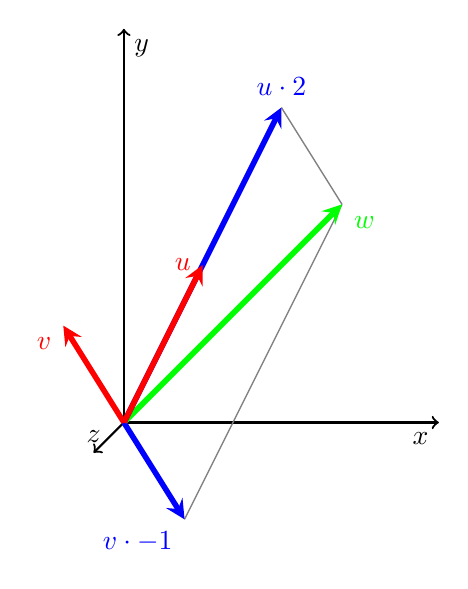
\begin{tikzpicture}
    	
	\draw[thick,->] (0,0,0) -- (4,0,0) node[anchor=north east]{$x$};
	\draw[thick,->] (0,0,0) -- (0,5,0) node[anchor=north west]{$y$};
    \draw[thick,->] (0,0,-5) -- (0,0,1) node[anchor=south]{$z$};
    
	\draw[line width=0.5pt,gray](2,4,0)--(2,2,-2) node[anchor=north east]{};
	\draw[line width=0.5pt,gray](0,-2,-2)--(2,2,-2) node[anchor=north east]{};
	
	\draw[line width=2pt,green,-stealth](0,0,0)--(2,2,-2) node[anchor=north west]{$\boldsymbol{w}$};    

	\draw[line width=2pt,blue,-stealth](0,0,0)--(2,4,0) node[anchor=south]{$\boldsymbol{u \cdot 2}$};
  	\draw[line width=2pt,blue,-stealth](0,0,0)--(0,-2,-2) node[anchor=north east]{$\boldsymbol{v \cdot -1}$};	
	\draw[line width=2pt,red,-stealth](0,0,0)--(1,2,0) node[anchor=east]{$\boldsymbol{u}$};
  	\draw[line width=2pt,red,-stealth](0,0,0)--(0,2,2) node[anchor=north east]{$\boldsymbol{v}$};
	
\end{tikzpicture}
\caption{Erzeugen eines neuen Vektors $w$ aus zwei linear unabhängigen Vektoren $v$ und $u$.}
\end{figure} \label{img:0}

\noindent In dem Beispiel der Grafik 1.1 ist $r = 2$ und $s = -1$. 



\subsubsection{ Betrag / Länge }

Der Betrag oder auch Länge eines Vektors ist gleich dem euklidischen Abstand der Punkte $A$ und $B$ im Raum. Zur berechnung nutzt man den Satz des Pythagoras an.

\begin{figure}[h]
\centering
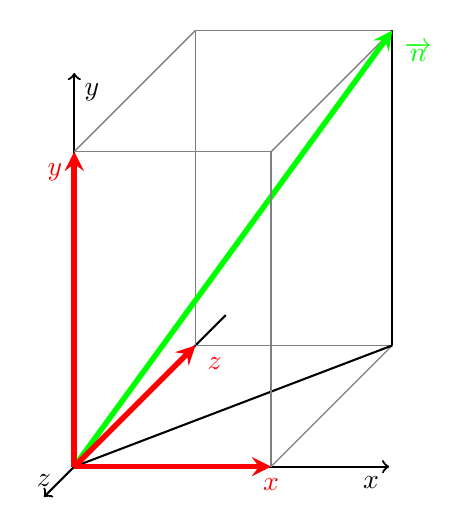
\begin{tikzpicture}
    	
	\draw[thick,->] (0,0,0) -- (4,0,0) node[anchor=north east]{$x$};
	\draw[thick,->] (0,0,0) -- (0,5,0) node[anchor=north west]{$y$};
    \draw[thick,->] (0,0,-5) -- (0,0,1) node[anchor=south]{$z$};
    
	\draw[line width=0.5pt,gray](2.5,0,0)--(2.5,0,-4) node[anchor=north east]{};
	\draw[line width=0.5pt,gray](0,0,-4)--(2.5,0,-4) node[anchor=north east]{};

	\draw[line width=0.5pt,gray](2.5,4,0)--(2.5,4,-4) node[anchor=north east]{};	
	\draw[line width=0.5pt,gray](0,4,-4)--(2.5,4,-4) node[anchor=north east]{};	
	\draw[line width=0.5pt,gray](0,0,-4)--(0,4,-4) node[anchor=north east]{};		
	\draw[line width=0.75pt,black](2.5,0,-4)--(2.5,4,-4) node[anchor=north east]{};	
	\draw[line width=0.5pt,gray](0,4,0)--(2.5,4,0) node[anchor=north east]{};
	\draw[line width=0.5pt,gray](0,4,0)--(0,4,-4) node[anchor=north east]{};
	
	\draw[line width=0.75pt,black](0,0,0)--(2.5,0,-4) node[anchor=center]{};	
	
	\draw[line width=2pt,green,-stealth](0,0,0)--(2.5,4,-4) node[anchor=north west]{$\boldsymbol{\overrightarrow{n}}$};    
     
	
	\someWinkel{2.5,0,0}{45}{135}
    
	\draw[line width=2pt,red,-stealth](0,0,0)--(2.5,0,0) node[anchor=north]{$\boldsymbol{x}$};
  	\draw[line width=2pt,red,-stealth](0,0,0)--(0,4,0) node[anchor=north east]{$\boldsymbol{y}$};
	\draw[line width=2pt,red,-stealth](0,0,0)--(0,0,-4) node[anchor=north west]{$\boldsymbol{z}$};
	
	\draw[line width=0.5pt,gray](2.5,0,0)--(2.5,4,0) node[anchor=north east]{};	
\end{tikzpicture}
\caption{Darstellung eines Vektors mit seinen Komponenten im drei dimensionalen Raum}
\end{figure}

\begin{align*}
	\vert \overrightarrow{x} \vert  = \sqrt{\sum_{k=1}^n x_k^2}
\end{align*} 



\subsection{Besondere Vektoren}

\subsubsection{ Nullvektor }

Der Nullvektor $ \overrightarrow{0} $ ist neutrale Element $ 0_V $  der Vektoraddition. Zudem ist er kein Vektor im traditionellem Sinn, da er keine Richtung besitzt und eine Länge von $0$ hat und somit eher als ein Punkt gesehen werden kann anstelle als ein Pfeil.


\subsubsection{ Einheitsvektor }

Ist jeder Vektor mit einer Länge von $\vert \overrightarrow{x}_0 \vert = 1 $.

\begin{align*}
\xhat = \overrightarrow{x_0} = \frac{1}{\vert \overrightarrow{x} \vert} \cdot \overrightarrow{x} 
\end{align*}

\section{Basis und Standardbasis}

Eine Basis ist eine Teilmenge eines Vektorraumes $ B \subset V $. Jeder Vektor aus $ V $ lässt sich als Linearkombination der Vektoren aus $ B $ darstellen. Eine Standardbasis oder auch kanonische Basis hat als Vektoren in $ B $ nur Einheitsvektoren $ \overrightarrow{e_n}$  $ \forall v \in B \ \vert v \vert = 1 $.

\begin{align*}
	\overrightarrow{x} = r_1 \cdot \overrightarrow{e_1}  + \cdots + r_n \cdot \overrightarrow{e_n} = 
	I_n \cdot 		
	\begin{pmatrix}
		r_1 \\ \vdots \\ r_n
	\end{pmatrix}
\end{align*}

\begin{figure}[h]
\centering
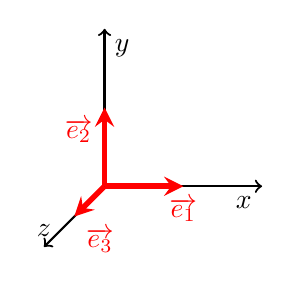
\begin{tikzpicture}
    	
	\draw[thick,->] (0,0,0) -- (2,0,0) node[anchor=north east]{$x$};
	\draw[thick,->] (0,0,0) -- (0,2,0) node[anchor=north west]{$y$};
    \draw[thick,->] (0,0,0) -- (0,0,2) node[anchor=south]{$z$};
    
	\draw[line width=2pt,red,-stealth](0,0,0)--(1,0,0) node[anchor=north]{$\boldsymbol{\overrightarrow{e_1}}$};
  	\draw[line width=2pt,red,-stealth](0,0,0)--(0,1,0) node[anchor=north east]{$\boldsymbol{\overrightarrow{e_2}}$};
	\draw[line width=2pt,red,-stealth](0,0,0)--(0,0,1) node[anchor=north west]{$\boldsymbol{\overrightarrow{e_3}}$};
	
\end{tikzpicture}
\caption{Darstellung der Einheitsvektoren in drei Dimensionen}
\end{figure}

Die Einheitsvektoren sind alle linear unabhängig von einander und alle haben eine Länge von $ 1 $ somit ist der Faktor vor einem Einheitsvektor gleich der Komponente des Vektors. %TODO clarification

\section{Raumtransformationen und Matritzen}
Man kann sich Matritzen unterschiedlich Vorstellen. Eine Möglichkeit ist vorstellung ein ein lineares Gleichungsystem die andere als lineare Raumtransformation.

\begin{figure}[h]
\centering
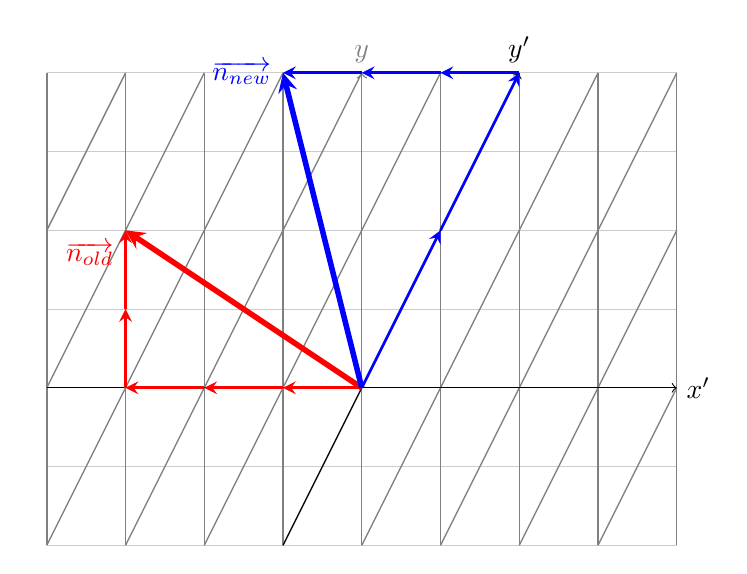
\begin{tikzpicture}

  \draw[thin,gray!40] (-4,-2) grid (4,4);
  \draw[->, line width=0.5pt,gray] (0,-2)--(0,4) node[above]{$y$};
  
  \draw[line width=0.5pt,gray](-4,-2)--(-1,4) node[anchor=north east]{};
  \draw[line width=0.5pt,gray](-4,0)--(-2,4) node[anchor=north east]{};
  \draw[line width=0.5pt,gray](-4,2)--(-3,4) node[anchor=north east]{};
  \draw[line width=0.5pt,gray](-3,-2)--(0,4) node[anchor=north east]{};
  \draw[line width=0.5pt,gray](-2,-2)--(1,4) node[anchor=north east]{};
  \draw[line width=0.5pt,gray](-1,-2)--(2,4) node[anchor=north east]{};
  
  \draw[line width=0.5pt,gray](0,-2)--(3,4) node[anchor=north east]{};
  \draw[line width=0.5pt,gray](1,-2)--(4,4) node[anchor=north east]{};
  \draw[line width=0.5pt,gray](2,-2)--(4,2) node[anchor=north east]{};
  \draw[line width=0.5pt,gray](3,-2)--(4,0) node[anchor=north east]{};
  
  
  \draw[line width=0.5pt,gray](-4,-2)--(-4,4) node[anchor=north east]{};
  \draw[line width=0.5pt,gray](-3,-2)--(-3,4) node[anchor=north east]{};
  \draw[line width=0.5pt,gray](-2,-2)--(-2,4) node[anchor=north east]{};
  \draw[line width=0.5pt,gray](-1,-2)--(-1,4) node[anchor=north east]{};
  \draw[line width=0.5pt,gray](0,-2)--(0,4) node[anchor=north east]{};
  \draw[line width=0.5pt,gray](1,-2)--(1,4) node[anchor=north east]{};
  \draw[line width=0.5pt,gray](2,-2)--(2,4) node[anchor=north east]{};
  \draw[line width=0.5pt,gray](3,-2)--(3,4) node[anchor=north east]{};
  \draw[line width=0.5pt,gray](4,-2)--(4,4) node[anchor=north east]{};

  \draw[->] (-4,0)--(4,0) node[right]{$x'$};
  \draw[->] (-1,-2)--(2,4) node[above]{$y'$};
  
  \draw[line width=1pt,red,-stealth](0,0)--(-1,0) node[anchor=west]{};
  \draw[line width=1pt,red,-stealth](-1,0)--(-2,0) node[anchor=west]{};
  \draw[line width=1pt,red,-stealth](-2, 0)--(-3,0) node[anchor=west]{};
 
  \draw[line width=1pt,red,-stealth](-3,0)--(-3,1) node[anchor=west]{}; 
  \draw[line width=1pt,red,-stealth](-3,1)--(-3,2) node[anchor=west]{};
  
  \draw[line width=1pt,blue,-stealth](0,0)--(1,2) node[anchor=west]{};
  \draw[line width=1pt,blue,-stealth](1,2)--(2,4) node[anchor=west]{};
  
  \draw[line width=1pt,blue,-stealth](2,4)--(1,4) node[anchor=west]{};
  \draw[line width=1pt,blue,-stealth](1,4)--(0,4) node[anchor=west]{};
  \draw[line width=1pt,blue,-stealth](0,4)--(-1,4) node[anchor=west]{};


  \draw[line width=2pt,red,-stealth](0,0)--(-3,2) node[anchor=north east]{$\boldsymbol{\overrightarrow{n_{old}}}$};
  \draw[line width=2pt,blue,-stealth](0,0)--(-1,4) node[anchor=east]{$\boldsymbol{\overrightarrow{n_{new}}}$};
\end{tikzpicture}
\caption{Darstellung einer Raumtransformation}
\end{figure}

\begin{align*}
	A = \begin{bmatrix}
		1 & 1 \\
		0 & 2
	\end{bmatrix}
\end{align*}

\subsection{Matrix Vektor Produkt}

Die druchführung einer Raumtransformation ist das Matrix-Vektor Produkt, wobei die Matrix die Raumtransformation beschreibt und der Vektor das zu transformierende Objekt repräsentiert. Mathematische Formulierung: $ K^{m \times n} \times K^n \rightarrow K^m $

\begin{align*}
	A \cdot \overrightarrow{n} = 
	\begin{bmatrix}
		1 & 1 \\
		0 & 2
	\end{bmatrix} \cdot 
	\begin{pmatrix}
		-3 \\ 2
	\end{pmatrix} = -3 \cdot 
	\begin{bmatrix}
		1 \\ 0	
	\end{bmatrix} + 2 \cdot
	\begin{bmatrix}
		1 \\ 2
	\end{bmatrix} =
	\begin{pmatrix}
		-1 \\ 4
	\end{pmatrix} 
\end{align*}

\noindent In einer Matrix werden also ein getragen wo die Einheitsvektoren der Standardbasis nach der Transformation landen.

\begin{itemize}
	\item Assoziativgesetzt 
	\begin{itemize}
		\item $ A \cdot ( B \cdot x ) = ( A \cdot B ) \cdot x $
		\item $ \alpha ( A \cdot x ) = ( \alpha \cdot A ) \cdot x = A \cdot (a \cdot x) $
	\end{itemize}	 
	\item Distributivgesetzt
	\begin{itemize}
		\item $ ( A + B ) \cdot x = A \cdot x + B \cdot x $
		\item $ A \cdot ( x + y ) = A \cdot x + A \cdot y $
	\end{itemize}	
\end{itemize}

\subsection{Matrix Produkt}

Sagen wir haben zwei Transformationen die wir nacheinander Ausführen diese beiden Transformationen können wir auch eine 




\section{Geraden}

\section{Skalarprodukt}

\section{Determinanten}

\section{Kreuzprodukt}

\section{Spatprodukt}

\section{Ebenen}

\section{Lagebeziehungen}



\subsubsection{ Begriffs Notationen}

\paragraph*{Ortsvektor} \( \overrightarrow{OX} \) ist definiert als der Vektor vom Koordinanten Ursprung der zum Punkt X zeigt. \newline

\subsection*{ Geraden }
Definiert als:

\( g \dots \overrightarrow{x} = \overrightarrow{a} \cdot r + \overrightarrow{b} \)

\subsection*{ Ebenen}

\paragraph*{Parameter Form } \( \varepsilon ... \overrightarrow{x} = \overrightarrow{a} \cdot r + \overrightarrow{b} \cdot s + \overrightarrow{OA} \)

\paragraph*{Koordinaten Form} \( \varepsilon ... d = \overrightarrow{p } \cdot \overrightarrow{n} \)

\paragraph*{Achsenabschnitts Form} \( \frac{x}{x_0} + \frac{y}{y_0} + \frac{z}{z_0} = 1 \)

\paragraph*{ Hesssche Normalform} \( 0 = \overrightarrow{n_0} \cdot( \overrightarrow{r} - \overrightarrow{p}) \)



\subsubsection*{ Lineare Raum Transformationen - Lineare Abbildung}

Betrachtung von Einheits Vekoren \( \ihat \land \jhat \vert n = 2\) wo sie nach der Transformation Landen. Transformation wird als Matrix geschrieben: \( \begin{bmatrix}
\ihat_0 & \jhat_0\\\
\ihat_1 & \jhat_1 
\end{bmatrix} \)  Der Trick für die Vorstellung ist das der zu Transformierende Vektor als Kombination von \( \ihat \land \jhat \) dargestellt werden kann. Das heißt \begin{equation}
\overrightarrow{v} = v_0 \cdot \ihat + v_1 \cdot \jhat \Rightarrow (\text{Transformed}) \overrightarrow{v} = v_0 \cdot (\text{Transformed}) \ihat + v_1 \cdot (\text{Transformed}) \jhat
\end{equation} Wenn wir uns im 2 Dimensionalen Bewegen aber das Konzept lässt sich auch simpel auf höhere Dimensionen übertragen. \newline

Notation: Matrizen wird beistens ein Großbuchstabe als Variable zugeordnet.

\subsubsection*{ Determinanten }

Der absolut Wert einer Determinate Gibt an um welchen Faktor bei einer Linearen Transformation sich die Fläche(oder Volumen \( n = 3\)) des betrachteten Felder ändert. Ist der Wert Null Drück die Lineare Abbildung den Raum auf einen kleinere Dimension. Ist die Determinate negativ wird der Raum gedreht. 



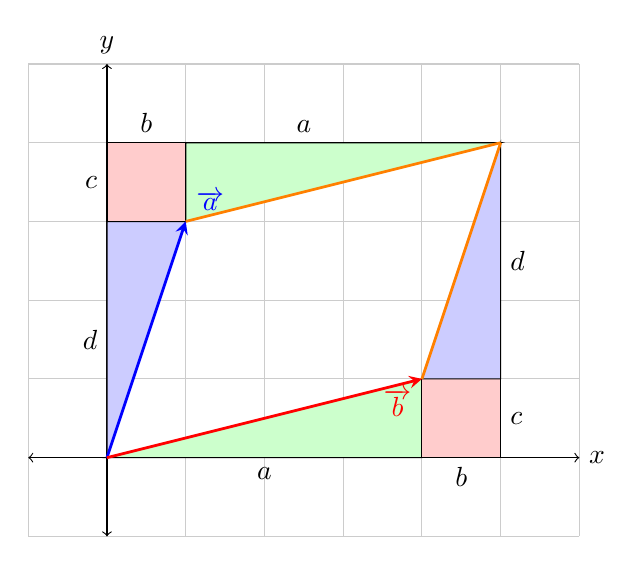
\begin{tikzpicture}
  \draw[thin,gray!40] (-1,-1) grid (6,5);
  \draw[<->] (-1,0)--(6,0) node[right]{$x$};
  \draw[<->] (0,-1)--(0,5) node[above]{$y$};
  
	\filldraw[fill=green!20] (0,0) node[anchor=north]{}
  -- (2,0) node[anchor=north]{$a$}
  -- (4,0) node[anchor=north]{}
  -- (4,1) node[anchor=south]{}
  -- cycle;
  
  	\filldraw[fill=red!20] (4,0) node[anchor=north]{}
  -- (4.5,0) node[anchor=north]{$b$}	
  -- (5,0) node[anchor=north]{}
  -- (5,0.5) node[anchor=west]{$c$}
  -- (5,1) node[anchor=south]{}
  -- (4,1) node[anchor=south]{}
  -- cycle;
  
  	\filldraw[fill=blue!20] (4,1) node[anchor=north]{}
  -- (5,1) node[anchor=north]{}
  -- (5,2.5) node[anchor=west]{$d$}
  -- (5,4) node[anchor=south]{}
  -- cycle;
  
  	\filldraw[fill=blue!20] (0,0) node[anchor=north]{}
  -- (0,1.5) node[anchor=east]{$d$}
  -- (0,3) node[anchor=north]{}
  -- (1,3) node[anchor=south]{}
  -- cycle;
  
	\filldraw[fill=red!20] (0,3) node[anchor=north]{}
  -- (0,3.5) node[anchor=east]{$c$}
  -- (0,4) node[anchor=north]{}
  -- (0.5,4) node[anchor=south]{$b$}
  -- (1,4) node[anchor=south]{}
  -- (1,3) node[anchor=south]{}
  -- cycle;
    
  	\filldraw[fill=green!20] (1,4) node[anchor=north]{}
  -- (2.5,4) node[anchor=south]{$a$}	
  -- (5,4) node[anchor=north]{}
  -- (1,3) node[anchor=south]{}
  -- cycle;
  
    \draw[line width=1pt,blue,-stealth](0,0)--(1,3) node[anchor=south west]{$\boldsymbol{\overrightarrow{a}}$};
  \draw[line width=1pt,red,-stealth](0,0)--(4,1) node[anchor=north east]{$\boldsymbol{\overrightarrow{b}}$};
  
  \draw[line width=1pt,orange](1,3)--(5,4) node[anchor=south west]{};
  \draw[line width=1pt,orange](4,1)--(5,4) node[anchor=north east]{};
	
	
\end{tikzpicture}

\begin{equation}
	det \bigg( \begin{bmatrix}
a & b\\\
c & d 
\end{bmatrix} \bigg) = (a+b) \cdot (d+c) - 2bc - db - ac = ad - bc
\end{equation}

\begin{equation} 
det \Bigg( \begin{bmatrix}
k_0 & v_0 & w_0 \\\
k_1 & v_1 & w_1 \\\
k_2 & v_2 & w_2
\end{bmatrix} \Bigg) = k_0 \cdot 	det \bigg( \begin{bmatrix}
v_1 & w_1\\\
v_2 & w_2 
\end{bmatrix} \bigg) - v_0 \cdot 	det \bigg( \begin{bmatrix}
k_1 & w_1\\\
k_2 & w_2 
\end{bmatrix} \bigg) + w_0 \cdot 	det \bigg( \begin{bmatrix}
k_1 & v_1\\\
k_2 & v_2 
\end{bmatrix} \bigg)
\end{equation}

\begin{equation} 
det \Bigg( \begin{bmatrix}
k_0 & v_0 & w_0 \\\
k_1 & v_1 & w_1 \\\
k_2 & v_2 & w_2
\end{bmatrix} \Bigg) = k_0 ( v_2 \cdot w_3 - v_3 \cdot w_2 ) + 
k_1 ( v_3 \cdot w_1 - v_1 \cdot w_3 )
+ k_2 (v_1 \cdot w_2 - v_2 \cdot w_1)
\end{equation}



\subsection*{ Scalar Produkt }

\begin{equation}
\overrightarrow{a} \cdot \overrightarrow{b} = \sum_{k=1}^n a_k \cdot b_k  = \vert \overrightarrow{a} \vert \cdot \vert \overrightarrow{b} \vert \cdot cos(\sphericalangle (\overrightarrow{a}, \overrightarrow{b} ))
\end{equation}
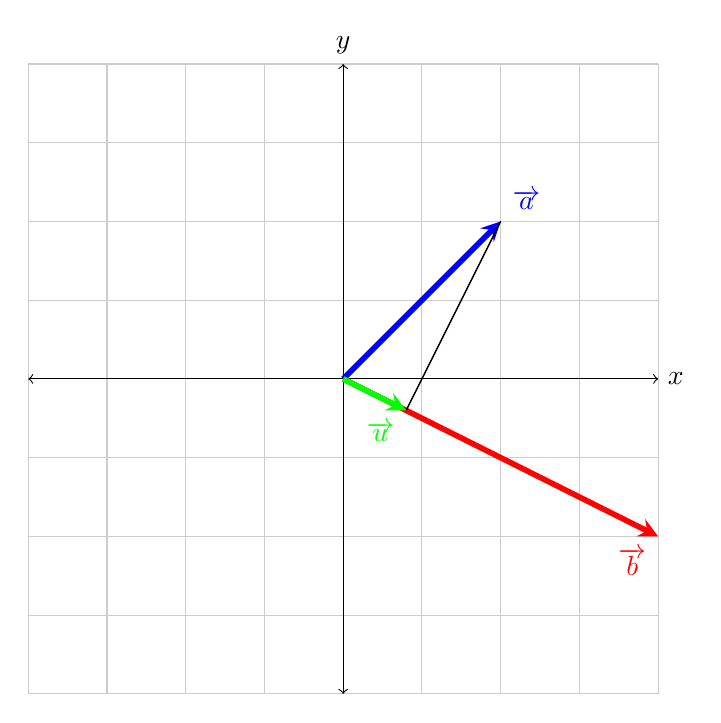
\begin{tikzpicture}
  \draw[thin,gray!40] (-4,-4) grid (4,4);
  \draw[<->] (-4,0)--(4,0) node[right]{$x$};
  \draw[<->] (0,-4)--(0,4) node[above]{$y$};
  \draw[line width=2pt,blue,-stealth](0,0)--(2,2) node[anchor=south west]{$\boldsymbol{\overrightarrow{a}}$};
  \draw[line width=2pt,red,-stealth](0,0)--(4,-2) node[anchor=north east]{$\boldsymbol{\overrightarrow{b}}$};
    \draw[line width=0.5pt,black](2,2)--(0.8,-0.4) node[anchor=north east]{};  
      \draw[line width=2pt,green,-stealth](0,0)--(0.8,-0.4) node[anchor=north east]{$\boldsymbol{\overrightarrow{u}}$};
  
\end{tikzpicture}

\( \overrightarrow{a} \cdot \overrightarrow{b} = \vert \overrightarrow{u} \vert \cdot \vert \overrightarrow{b} \vert \Rightarrow \vert \overrightarrow{u} \vert =  cos(\sphericalangle (\overrightarrow{a}, \overrightarrow{b} )) \cdot \vert \overrightarrow{a} \vert \)

Wobei \( \overrightarrow{b} \) Immer der Vektor ist auf dem \( \overrightarrow{u} \) Projeziert wird. \newline 

Das Dot Product kann aber auch als ein Matrix Vector produkt verstanden werden wobei die Lineare Abbildung alles auf eine Achse zusammen presst. Somit ist diese Matrix immer eine \( ( 1 \times n ) \) Matrix weil wir zu Faul sind die Nullen mit zuschreiben.

\begin{equation} 
\begin{bmatrix}
\ihat_0 & \jhat_0
\end{bmatrix}  
\cdot 
\begin{pmatrix}
x_1 \\ x_2
\end{pmatrix} = \ihat_0 \cdot x_1 + \jhat_0 \cdot x_2 
\end{equation}


Note für Verständniss: \( \begin{bmatrix}
\ihat_0 & \jhat_0
\end{bmatrix}   \) Kann hier als Rotierte Achse Verstanden werden die Anderen Vektoren wird auf diese Achse Projeziert.

\subsection*{ Kreuz Produkt} 

\subsubsection*{ In 2 Dimensions}

\begin{equation}
	 \begin{pmatrix}
	 	a  \\\
	 	b
	 \end{pmatrix} \times 	 \begin{pmatrix}
	 	c  \\\
	 	d
	 \end{pmatrix} = det \bigg( \begin{bmatrix}
	 	a & c \\\
	 	b & d
	 \end{bmatrix} \bigg) = a \cdot c - b \cdot d
\end{equation}

\subsubsection*{In 3 Dimensions }

In \( n = 3 \) Dimensionen .
\( \overrightarrow{a} \times \overrightarrow{b} = \begin{pmatrix}
	a_3 \cdot b_2 - a_2 \cdot b_3 \\ a_1 \cdot b_3 - a_3 \cdot b_1 \\ a_2 \cdot b_1 - a_1 \cdot b_2
\end{pmatrix} \) 

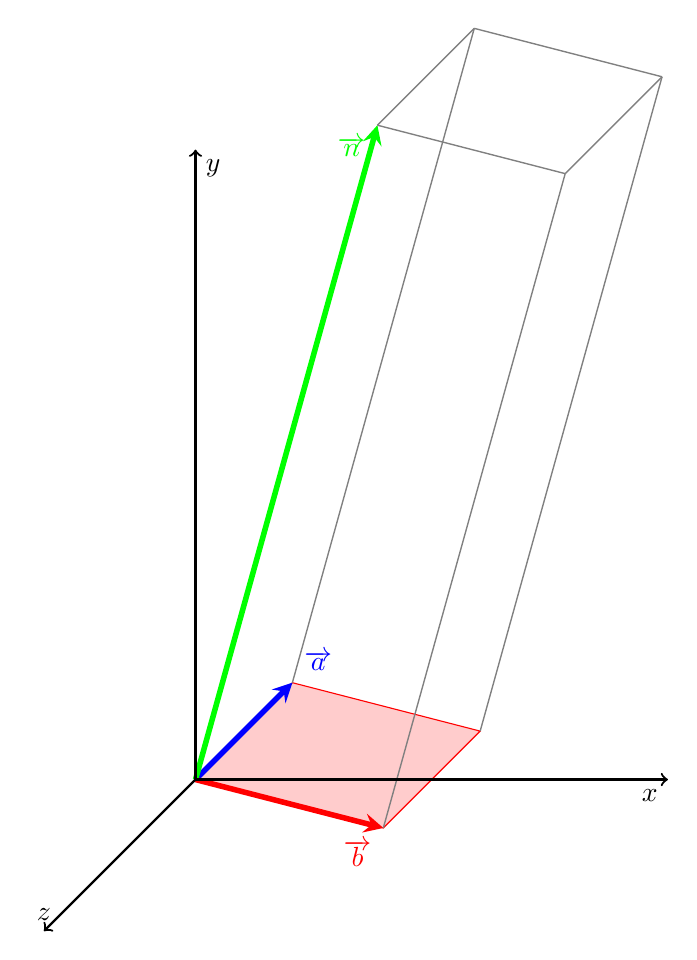
\begin{tikzpicture}[scale=1]

	    
    
    \def\x{.5}
    \filldraw[
        draw=red,%
        fill=red!20,%
    ]          (0,0,0)
            -- (2,2,2)
            -- (4,1,1)
            -- (2,-1,-1)
            -- cycle;
            
	\draw[line width=2pt,blue,-stealth](0,0,0)--(2,2,2) node[anchor=south west]{$\boldsymbol{\overrightarrow{a}}$};
  	\draw[line width=2pt,red,-stealth](0,0,0)--(2,-1,-1) node[anchor=north east]{$\boldsymbol{\overrightarrow{b}}$};
	\draw[line width=2pt,green,-stealth](0,0,0)--(0,6,-6) node[anchor=north east]{$\boldsymbol{\overrightarrow{n}}$};
	
	\draw[line width=0.5pt,gray](2,2,2)--(2,8,-4) node[anchor=north east]{};
	
	\draw[line width=0.5pt,gray](2,-1,-1)--(2,5,-7) node[anchor=north east]{};
	
	\draw[line width=0.5pt,gray](4,1,1)--(4,7,-5) node[anchor=north east]{};
	\draw[line width=0.5pt,gray](0,6,-6)--(2,8,-4) node[anchor=north east]{};
	\draw[line width=0.5pt,gray](2,8,-4)--(4,7,-5) node[anchor=north east]{};
	\draw[line width=0.5pt,gray](4,7,-5)--(2,5,-7) node[anchor=north east]{};
	\draw[line width=0.5pt,gray](2,5,-7)--(0,6,-6) node[anchor=north east]{};	
	\draw[thick,->] (0,0,0) -- (6,0,0) node[anchor=north east]{$x$};
	\draw[thick,->] (0,0,0) -- (0,8,0) node[anchor=north west]{$y$};
    \draw[thick,->] (0,0,0) -- (0,0,5) node[anchor=south]{$z$};
\end{tikzpicture}

Für die Herleitung das Spatprodukt ist gleich der Determinante der \( ( 3 \times 3 ) \) Matrix aus dem 3. Vektor des Spat Produkt und den beiden Richtungsvektoren \( \overrightarrow{a} \land \overrightarrow{b} \)

\begin{equation}
	\begin{pmatrix}
		 p_1 \\\ p_2 \\\ p_3
	\end{pmatrix} \cdot \begin{pmatrix}
		 x \\\ y \\\ z
	\end{pmatrix} = det \Bigg( \begin{bmatrix}
		x & v_1 & w_1 \\\
		y & v_2 & w_2 \\\
		z & v_3 & w_3 
	\end{bmatrix} \Bigg)
\end{equation}

\begin{equation}
	p_1 \cdot x + p_2 \cdot y + p_3 \cdot z = x ( v_2 \cdot w_3 - v_3 \cdot w_2 ) + 
y ( v_3 \cdot w_1 - v_1 \cdot w_3 )
+ z (v_1 \cdot w_2 - v_2 \cdot w_1)
\end{equation}

\begin{equation}
\overrightarrow{p} = \begin{pmatrix}
v_2 \cdot w_3 - v_3 \cdot w_2 \\\
v_3 \cdot w_1 - v_1 \cdot w_3 \\\
v_1 \cdot w_2 - v_2 \cdot w_1
\end{pmatrix}
\end{equation}

Der Flächeninhalt der von \( \overrightarrow{a} \land  \overrightarrow{b} \) eingeschlossenen Fläche ist \( \vert \overrightarrow{a} \times \overrightarrow{b} \vert \)

\subsection*{ Spatprodukt }

\( (\overrightarrow{a} \times \overrightarrow{b}) \cdot \overrightarrow{c} = V \)

\subsection*{ Punkt Ebene Beziehung }

\( 0 = \overrightarrow{n} \cdot (\overrightarrow{x}- \overrightarrow{p}) \land \overrightarrow{x} = \overrightarrow{r} + t \cdot \overrightarrow{n}  \land \overrightarrow{RF} = t \cdot \overrightarrow{n} \land \vert \overrightarrow{RF} \vert = d \)
Gerade in die Ebene einsetzten und nach der Laufvariable der geraden t umstellen ergibt. \( t = \frac{ \overrightarrow{n} \cdot ( \overrightarrow{p} - \overrightarrow{r}) }{ \vert \overrightarrow{n} \vert ^2} \) Wenn wir das jetzt in \( d = \vert t \cdot \overrightarrow{n } \vert \) einsetzen erhalten wir: \( d = \frac{\vert \overrightarrow{n} \cdot ( \overrightarrow{p} - \overrightarrow{r} ) \vert }{\vert \overrightarrow{n} \vert } \) ähnelt der Hesschen Normal Form \( \Rightarrow d = \vert \overrightarrow{n_0} \cdot ( \overrightarrow{r} - \overrightarrow{p} ) \vert \) Das absolut weil ein Abstand immer positiv ist.

\subsection*{ Lagebeziehungs Verschiedener Objekte } 

Windschief: \( g_1 \cap g_2 = \emptyset \land \text{linear unabhängig} \)


\paragraph*{ Gerade - Gerade } (Windschief , \( \parallel \), \( \equiv \), \( g_1 \cap g_2 = S \))

\paragraph*{ Gerade - Ebene} (\( \parallel \),\( \equiv \), \( g \in \varepsilon \), \( g \cap \varepsilon = S \))

\paragraph*{ Ebene - Ebene} (\( \parallel \), \( \equiv \), \( \varepsilon_1 \cap \varepsilon_2 = g \))

\subsubsection*{ Coole Ideen die ich mir Merken sollte}

Der Richtungs Vektor der Schnittgeraden zweier Ebenen ist das Kreuzprodukt der Beiden Normal Vektoren. \newline

Richtungs Vektor einer Geraden als Normalen Vektoren einer Ebene betrachten für Berechnungen wie min Abstand zweier Windschiefer geraden.

